\section{Efficient Grid Size Reduction}
\label{gridred}
\begin{figure}
\centering
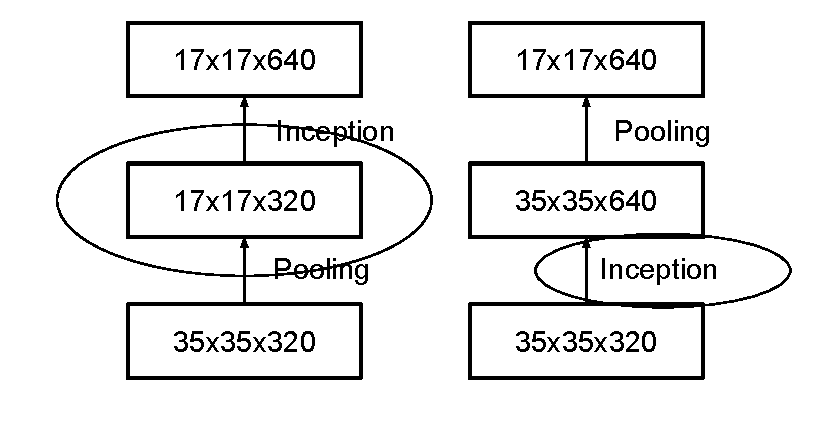
\includegraphics[width=\linewidth]{gridreduction}
\caption{Two alternative ways of reducing the grid size. The solution on the
  left violates the principle~\ref{nobottlenecks} of
  not introducing an representational bottleneck from Section~\ref{principles}.
  The version on the right is $3$ times more expensive computationally.
}
\label{fig:gridreduction}
\end{figure}
\begin{figure}
\centering
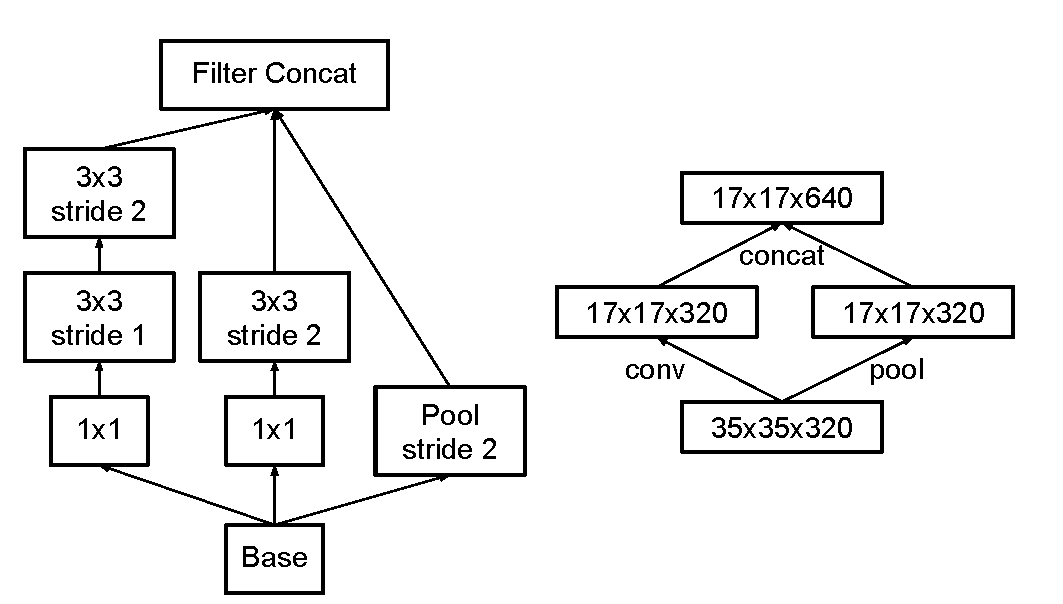
\includegraphics[width=\linewidth]{hybridreduction}
\caption{Inception module that reduces the grid-size while expands the filter
  banks. It is both cheap and avoids the representational bottleneck as is
  suggested by principle~\ref{nobottlenecks}. 
  The diagram on the right represents the same solution but from the
  perspective of grid sizes rather than the operations.}
\label{fig:hybridreduction}
\end{figure}
Traditionally, convolutional networks used some pooling operation to decrease
the grid size of the feature maps. In order to avoid a representational
bottleneck, before applying maximum or average pooling the activation
dimension of the network filters is expanded.
For example, starting a $d\times d$ grid
with $k$ filters, if we would like to arrive at a
$\frac{d}{2}\times \frac{d}{2}$ grid with $2k$ filters,
we first need to compute a stride-1 convolution with $2k$
filters and then apply an additional pooling step. This means that the overall
computational cost is dominated by the expensive convolution on the larger grid
using $2d^2k^2$ operations. One possibility would be to switch to pooling with
convolution and therefore resulting in $2(\frac{d}{2})^2k^2$ reducing the
computational cost by a quarter. However, this creates a representational
bottlenecks as the overall dimensionality of the representation drops to
$(\frac{d}{2})^2k$ resulting in less expressive networks (see
Figure~\ref{fig:gridreduction}).
Instead of doing so, we suggest another variant the reduces the computational
cost even further while removing the representational bottleneck.
(see Figure~\ref{fig:hybridreduction}).
We can use two parallel stride 2 blocks: $P$ and $C$. $P$ is a pooling layer
(either average or maximum pooling) the activation, both of them are stride
$2$ the filter banks of which are concatenated as in
figure~\ref{fig:hybridreduction}.
\begin{table}
{\small
 \begin{center}
   \begin{tabular}[H]{|l|c|c|}
   \hline
   {\bf type} & \stackanchor{\bf patch size/stride}{or remarks} & {\bf input size} \\
   \hline\hline
   conv & $3{\times}3/2$ & $299{\times}299{\times}3$ \\
   \hline
    conv & $3{\times}3/1$ & $149{\times}149{\times}32$ \\
   \hline
   conv padded & $3{\times}3/1$ & $147{\times}147{\times}32$ \\
   \hline
   pool & $3{\times}3/2$ & $147{\times}147{\times}64$ \\
   \hline
   conv & $3{\times}3/1$ & $73{\times}73{\times}64$ \\
   \hline
   conv & $3{\times}3/2$ & $71{\times}71{\times}80$ \\
   \hline
   conv & $3{\times}3/1$ & $35{\times}35{\times}192$ \\
   \hline
   $3\times$Inception & As in figure~\ref{fig:inceptionv2} & $35{\times}35{\times}288$ \\
   \hline
   $5\times$Inception & As in figure~\ref{fig:inceptionv3} & $17{\times}17{\times}768$ \\
   \hline
   $2\times$Inception & As in figure~\ref{fig:inceptionv4} & $8{\times}8{\times}1280$ \\
   \hline
   pool & $8\times 8$ & $8\times 8\times 2048$ \\
   \hline
   linear & logits & $1\times 1\times 2048$ \\
   \hline
   softmax & classifier & $1\times 1\times 1000$ \\
   \hline
   \end{tabular}
 \end{center}
 }
\caption{The outline of the proposed network architecture.
  The output size of each module is the input size of the next one.
  We are using variations of reduction technique depicted
  Figure~\ref{fig:hybridreduction} to reduce the grid sizes between the
  Inception blocks whenever applicable.
  We have marked the convolution with $0$-padding,
  which is used to maintain the grid size. $0$-padding is also used
  inside those Inception modules that do not reduce the grid size.
  All other layers do not use padding. The various filter bank
  sizes are chosen to observe principle~\ref{balance} from
  Section~\ref{principles}.
}
\label{table:stem}
\end{table}

\section{Inception-v2}
\label{revisited}
Here we are connecting the dots from above and propose a new
architecture with improved performance on the ILSVRC 2012
classification benchmark.
The layout of our network is given in table~\ref{table:stem}.
Note that we have factorized the traditional $7\times 7$ convolution into
three $3\times 3$ convolutions based on the same ideas as described in
section~\ref{factorizing}.
For the Inception part of the network, we have $3$ traditional
inception modules at  the $35\times 35$ with $288$ filters each.
This is reduced to a $17\times 17$ grid with $768$ filters using the
grid reduction technique described in section \ref{gridred}. This is
is followed by $5$ instances of the factorized inception modules as
depicted in figure~\ref{fig:inceptionv2}. This is reduced to a $8\times 8\times 1280$
grid with the grid reduction technique depicted in figure \ref{fig:hybridreduction}.
At the coarsest $8\times 8$ level, we have two Inception modules as depicted
in figure~\ref{fig:inceptionv3}, with a concatenated output filter bank size of
2048 for each tile. The detailed structure of the
network, including the sizes of filter banks inside the Inception modules,
is given in the supplementary material, given in the {\tt model.txt} that is in
the tar-file of this submission. However, we have observed that
the quality of the network is relatively stable to variations
as long as the principles from Section~\ref{principles} are observed.
Although our network is $42$ layers deep, our computation cost is only
about $2.5$ higher than that of GoogLeNet and it is still much more efficient than
VGGNet.

